\chapter{Implementacija i korisničko sučelje}
		
		
		\section{Korištene tehnologije i alati}
			 
			 \noindent \underbar{\textbf{MiKTeX}}
			 \begin{packed_item}
			 	\item  \textbf{Opis:} MiKTeX je besplatna distribucija otvorenog koda TeX/LaTeX sustava za Microsoft Windows.
			 	\item  \textbf{Mjesto primjene:} Projektna dokumentacija
			 	\item  \textbf{Poveznica:} https://miktex.org/
			 \end{packed_item}
		
			\noindent \underbar{\textbf{Visual paradigm}}
			\begin{packed_item}
				\item  \textbf{Opis:} Visual paradigm je UML CASE alat koji se koristi za stvaranje UML dijagrama.
				\item  \textbf{Mjesto primjene:} Projektna dokumentacija
				\item  \textbf{Poveznica:} https://www.visual-paradigm.com/
			\end{packed_item}
		
			\noindent \underbar{\textbf{Java Spring Framework}}
			\begin{packed_item}
				\item  \textbf{Opis:} Java Spring Framework je razvojni okvir otvorenog koda za stvaranje samostalnih aplikacija koje se pokreću na Java Virtual Machine-u (JVM).
				\item  \textbf{Mjesto primjene:} Web aplikacija - backend
				\item  \textbf{Poveznica:} https://spring.io/projects/spring-framework/
			\end{packed_item}
		
			\noindent \underbar{\textbf{React}}
			\begin{packed_item}
				\item  \textbf{Opis:} React je besplatna JavaScript biblioteka otvorenog koda za izgradnju korisničkih sučelja.
				\item  \textbf{Mjesto primjene:} Web aplikacija - frontend
				\item  \textbf{Poveznica:} https://reactjs.org/
			\end{packed_item}
		
			\noindent \underbar{\textbf{Leaflet}}
			\begin{packed_item}
				\item  \textbf{Opis:} Leaflet je JavaScript biblioteka otvorenog koda koja se koristi za izradu web aplikacija s kartama.
				\item  \textbf{Mjesto primjene:} Web aplikacija - frontend
				\item  \textbf{Poveznica:} http://leafletjs.com/
			\end{packed_item}
		
			\noindent \underbar{\textbf{Heroku}}
			\begin{packed_item}
				\item  \textbf{Opis:} Heroku je cloud platforma kao usluga (PaaS) koja podržava nekoliko programskih jezika.
				\item  \textbf{Mjesto primjene:} Puštanje aplikacije u pogon
				\item  \textbf{Poveznica:} https://www.heroku.com/
			\end{packed_item}
			
			\noindent \underbar{\textbf{Selenium}}
			\begin{packed_item}
				\item  \textbf{Opis:} Selenium je projekt otvorenog koda za niz alata i knjižnica čiji je cilj podrška automatizaciji web preglednika. Koristi se za testiranje.
				\item  \textbf{Mjesto primjene:} Ispitivanje programskog rješenja
				\item  \textbf{Poveznica:} https://www.selenium.dev/
			\end{packed_item}
			
			\noindent \underbar{\textbf{JUnit}}
			\begin{packed_item}
				\item  \textbf{Opis:} JUnit je okvir za programski jezik Java koji služi za ispitivanje jedinica.
				\item  \textbf{Mjesto primjene:} Ispitivanje programskog rješenja
				\item  \textbf{Poveznica:} https://junit.org/
			\end{packed_item}
			\eject 
		
	
		\section{Ispitivanje programskog rješenja}
			
			\subsection{Ispitivanje komponenti}
			\begin{packed_enum}
			
				\item Test stvara novog korisnika i provjerava postoji li korisnik s istim imenom u repozitoriju, zatim ispituje potvrđivanje tog korisnika.
				\begin{lstlisting}
public void testUser() throws Exception {
	userService.createUser(new User(null, "test1", "", "secret", "Test", "Test", "", "", "policeman", false));
	
	assertTrue(userRepo.findUserByUserName("test1").isPresent());
	User user = userRepo.findUserByUserName("test1").get();
	assertFalse(user.isConfirmed());
	assertTrue(userService.confirmUser(user.getId()));
	user = userRepo.findById(user.getId()).get();
	assertTrue(user.isConfirmed());
}
				\end{lstlisting}
				\item Test stvara potvrđene korisnike s ulogama vatrogasca i dispečera, zatim provjerava jesu li stvoreni ostali potrebni entiteti (Responder, Dispatcher) i jesu li ispravno povezani.
				\begin{lstlisting}
public void testRole() throws Exception {
	User user1 = userService.createUser(new User(null, "test2", "", "secret", "Test", "Test", "", "", "fireman", true));
	Responder responder = responderService.findByUserId(user1.getId()).get();
	assertEquals("test2", responder.getUserName());
	assertEquals(responder.getUser_id(), user1.getId());
	
	User user2 = userService.createUser(new User(null, "test3", "", "secret", "Test", "Test", "", "", "dispatcher", true));
	assertEquals(user2.getId(), dispatcherService.listAll().get(0).getUser());
}
				\end{lstlisting}
				\item Test otvara akciju, provjerava ispravnost dodavanja spasioca i zatvaranja akcije.
				\begin{lstlisting}
public void testAction() throws Exception {
	User user = userService.createUser(new User(null, "test4", "", "secret", "Test", "Test", "", "", "doctor", true));
	Responder responder = responderService.findByUserId(user.getId()).get();
	
	Action act = new Action();
	act.setName("test action");
	act.setDescription("test...");
	act.setTeam(new ArrayList<Responder>());
	act.setTasks(new ArrayList<Task>());
	actionService.createAction(act);
	
	assertTrue(actionService.addResponderToAction(responder.getId(), act.getId()));
	assertTrue(actionService.displayResponders(act.getId()).contains(responder));
	
	assertTrue(actionService.closeAction(act.getId()));
}
				\end{lstlisting}
				\item Test stvara novu stanicu i dodaje joj dva spasioca (voditelja i člana), zatim provjerava uspješnost tih funkcionalnosti.
				\begin{lstlisting}
public void testStation() throws Exception {
	User user1 = userService.createUser(new User(null, "test5", "", "secret", "Test", "Test", "", "", "doctor", true));
	Responder director = responderService.findByUserId(user1.getId()).get();
	User user2 = userService.createUser(new User(null, "test6", "", "secret", "Test", "Test", "", "", "doctor", true));
	Responder responder = responderService.findByUserId(user2.getId()).get();
	
	Station station = stationService.createStation(new Station("Test station", director.getId(),
	locationService.createLocation(new Location()).getId(), StationType.HOSPITAL));
	station.setMembers(new ArrayList<Long>());
	station = stationService.addMember(station.getId(), responder.getId());
	
	assertTrue(station.getMembers().contains(responder.getId()));
	assertEquals(station.getDirector_id(), director.getId());
}
				\end{lstlisting}
				\item Test stvara novu akciju, dodaje joj zadatak i zadatku dodaje komentar. Test ispituje navedene funkcionalnosti pomoću povratnih vrijednosti.
				\begin{lstlisting}
public void testTask() throws Exception {
	User user = userService.createUser(new User(null, "test7", "", "secret", "Test", "Test", "", "", "policeman", true));
	
	Action act = new Action();
	act.setName("test action");
	act.setDescription("test...");
	act.setTeam(new ArrayList<Responder>());
	act.setTasks(new ArrayList<Task>());
	actionService.createAction(act);
	
	Task task = taskService.save(new Task(null, "test task", user.getId(), new ArrayList<Long>(), new ArrayList<Comment>()));
	assertEquals(user.getId(), task.getResponder_id());
	assertTrue(actionService.addTask(task.getId(), act.getId()));
	assertTrue(taskService.addComment(new Comment(), task.getId()));
}
				\end{lstlisting}
				\item Test dodaje spasioca stanici kojoj ne pripada i pritom očekuje IllegalArgumentException. Funkcionalnost nije implementirana.
				\begin{lstlisting}
public void testWrongStationType() throws Exception {
	User user1 = userService.createUser(new User(null, "test8", "", "secret", "Test", "Test", "", "", "policeman", true));
	Responder director = responderService.findByUserId(user1.getId()).get();
	User user2 = userService.createUser(new User(null, "test9", "", "secret", "Test", "Test", "", "", "doctor", true));
	Responder responder = responderService.findByUserId(user2.getId()).get();
	
	Station station = stationService.createStation(new Station("Test station 2", director.getId(),
	locationService.createLocation(new Location()).getId(), StationType.POLICE));
	station.setMembers(new ArrayList<Long>());
	
	assertThrows(IllegalArgumentException.class, () -> stationService.addMember(station.getId(), responder.getId()));
}
				\end{lstlisting}
			\end{packed_enum}
			
			\begin{figure}[H]
				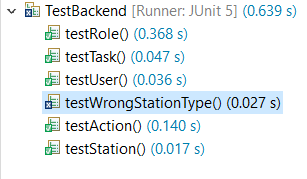
\includegraphics[scale=0.9]{slike/test.png}
				\centering
				\caption{Rezultati testova}
				\label{fig:test}
			\end{figure}
			
			testWrongStationType() je jedini test koji ne prolazi uspješno, jer funkcionalnost koju ispituje nije implementirana.
		
			\subsection{Ispitivanje sustava}
			
			 Za pokretanje Selenium testova, potrebno je imati ekstenziju na pregledniku za pokretanje testova. Testovi se pokreću redom označenim brojevima.
			 \begin{itemize}
			 	\item 1RegisterTest - Registrira 2 nova korisnika.
			 	\item 2AdminConfirmAndCreateStation - Potvrđuje dva nova korisnika i stvara stanicu.
			 	\item 3VoditeljTest - Prijava voditelja i dodavanje drugog korisnika u stanicu.
			 	\item 4DispatcherAction - Prijava dispatchera i stvaranje i zadavanje akcije.
			 	\item LoginFAIL - Neuspješna prijava u sustav.
			 \end{itemize}

			
			\eject 
		
		
		\section{Dijagram razmještaja}
			
			\textbf{\textit{dio 2. revizije}}
			
			 \begin{figure}[H]
			 	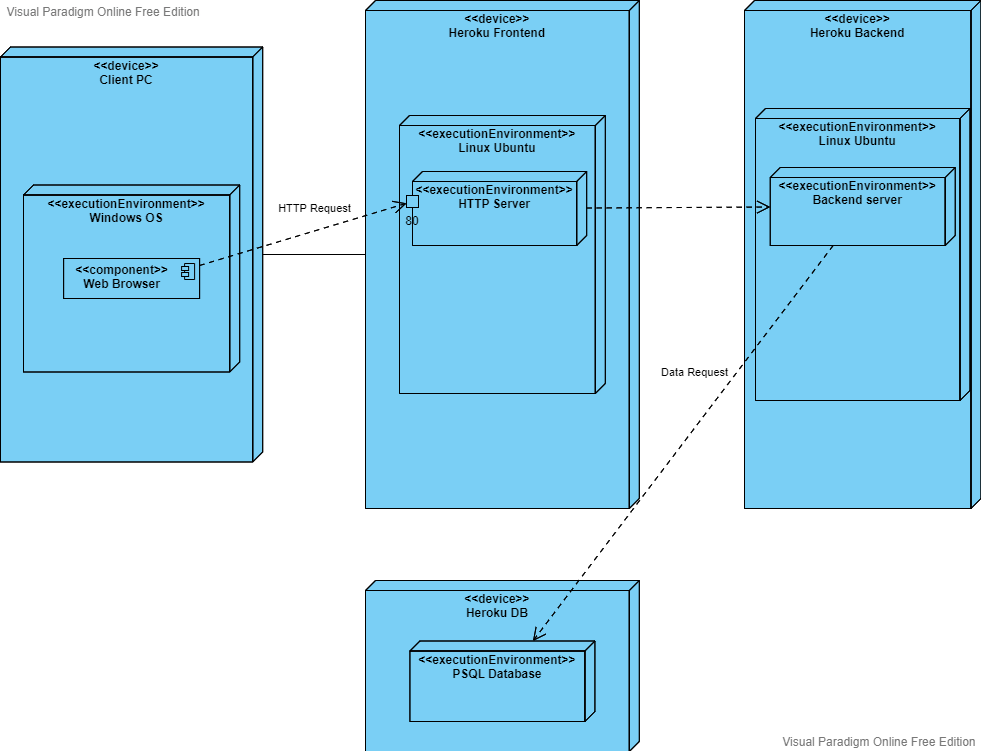
\includegraphics[scale=0.45]{slike/razmjestaj.PNG}
			 	\centering
			 	\caption{Dijagram razmještaja}
			 	\label{fig:razmještaj}
			 \end{figure}
			Prikaz dijagrama razmještaja. U sustavu postoje klijent, frontend server, backend server i baza podataka.
			
			\eject 
		
		\section{Upute za puštanje u pogon}
		
			\subsection{Priprema za puštanje u pogon}
			
			Kako bi aplikacija radila potrebno je instalirati NodeJs, Maven i Javu (minimum verzija 11). Moguće da je također potrebno postaviti sustavske varijable okruženja što se može napraviti  odlaskom u Control Panel -> System and Security -> System -> Advanced System Settings -> Enviromental Variables gdje u dolnjem izborniku treba pronaći PATH i ukoliko nedostaje dodati relativanputdonodejs/nodejs i relativan putdomavena/bin.
			
			\subsection{Puštanje u pogon}
			
			Kada su programi instalirani, potrebno je upaliti command prompt konzolu koja se može pokrenuti upisivanjem cmd u Windowsov pretraživač i premijestiti se u lokaciju projekta (korištenjem cd (path) naredbe). Zatim se premijestite u IzvorniKod/frontend te tamo pokrenite naredbu npm install koja će instalirati potrebne node pakete. Nakon toga pokrenite naredbu npm start koja će otvoriti vas browser i pokrenuti frontend.
			

		
				\begin{figure}[H]
					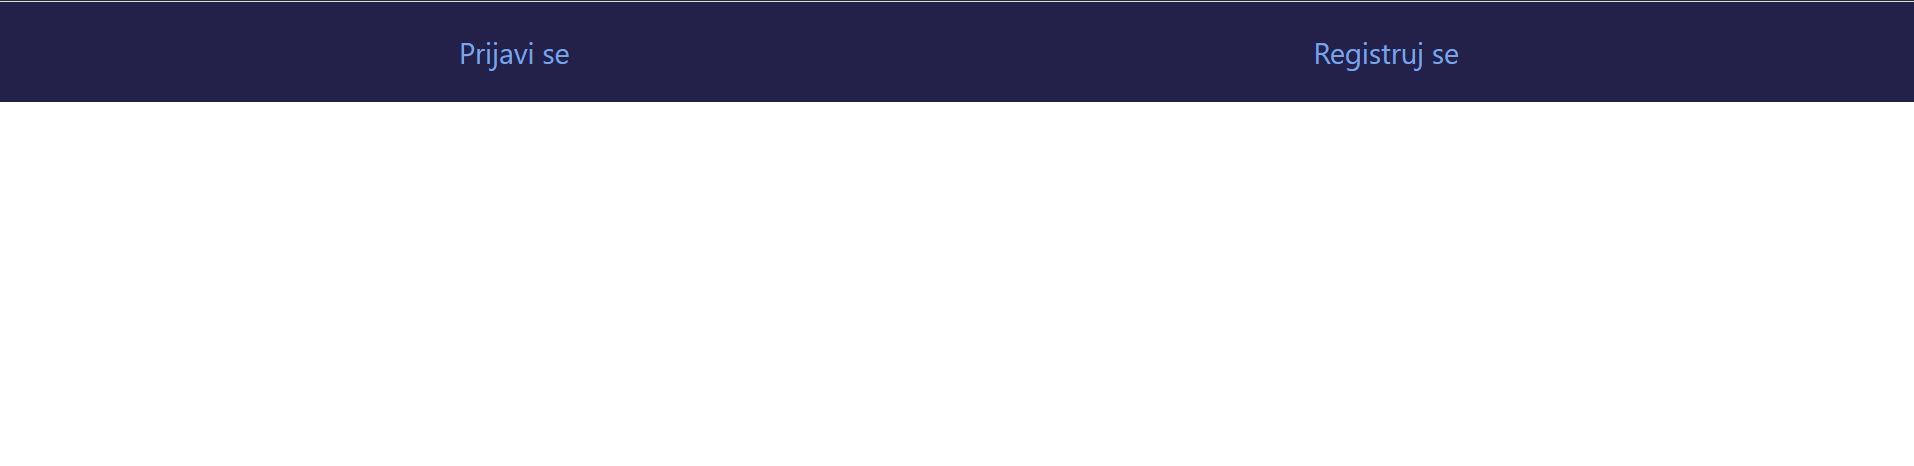
\includegraphics[scale=0.3]{slike/browser.png}
					\centering
					\caption{Otvoreni browser}
					\label{fig:test4}
				\end{figure}
		
				\begin{figure}[H]
					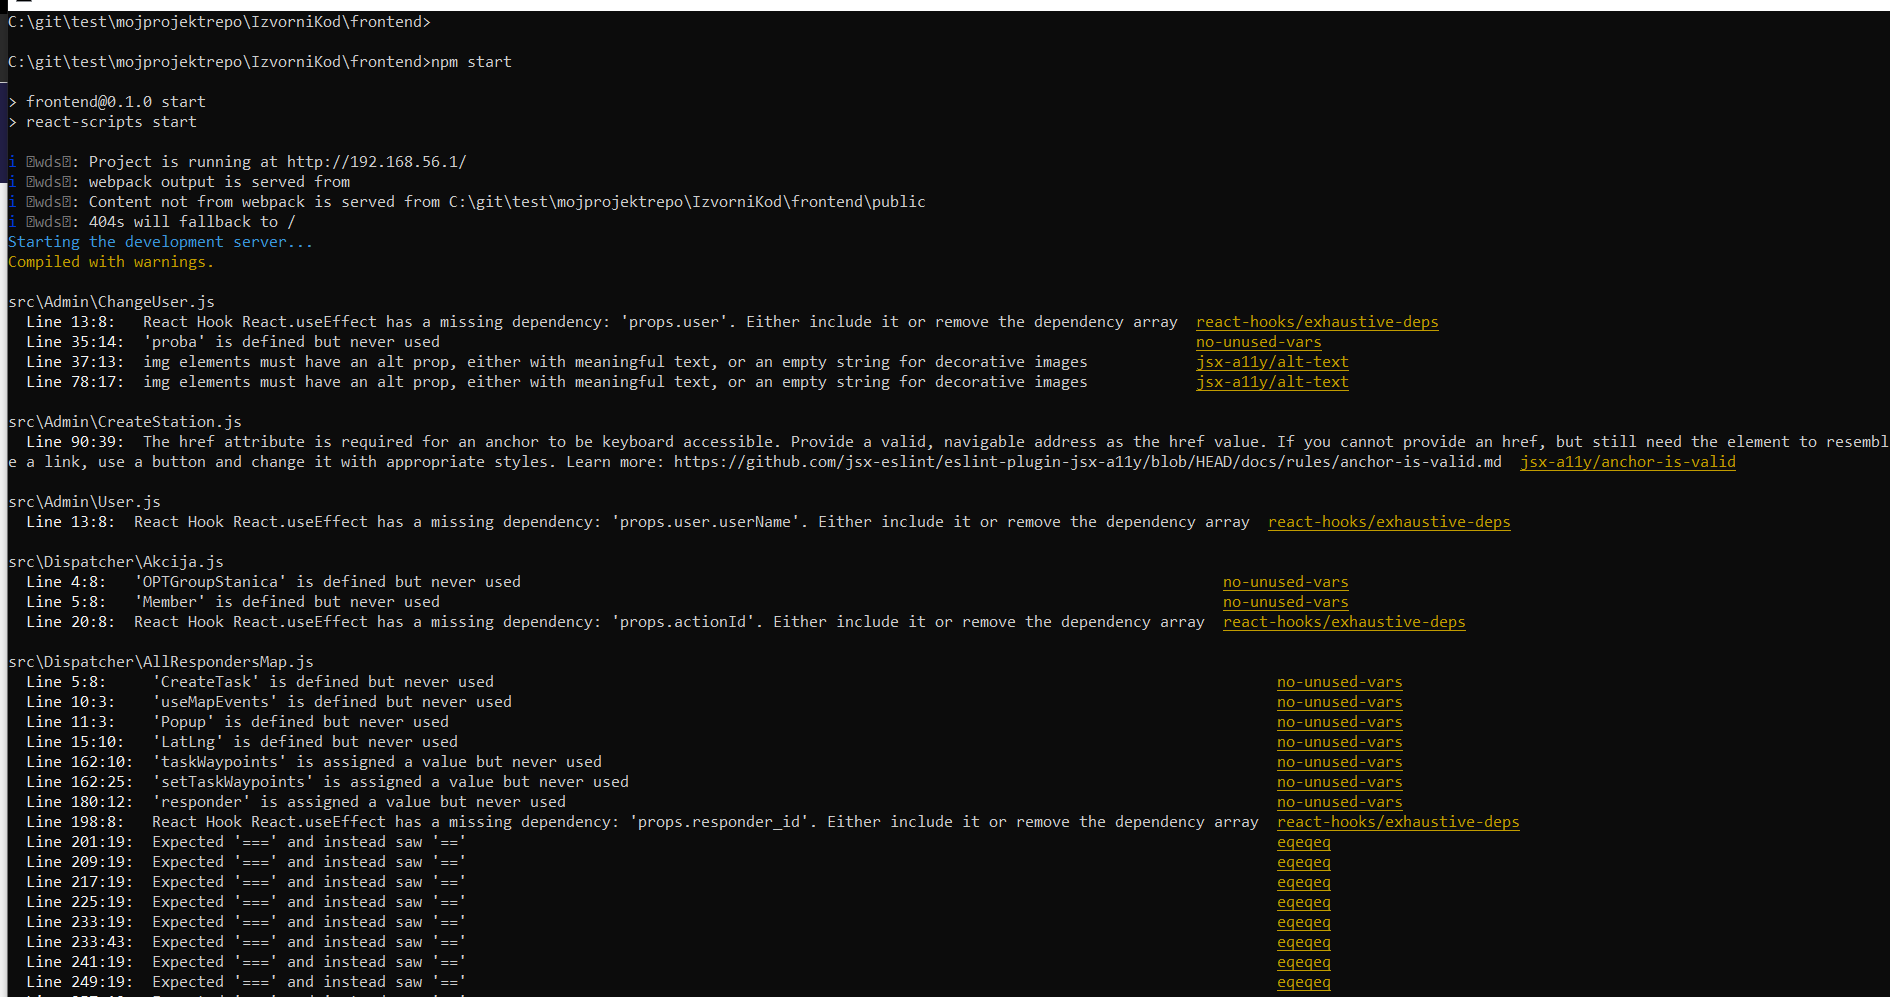
\includegraphics[scale=0.3]{slike/pokretanje_frontenda.png}
					\centering
					\caption{Pokretanje frontenda iz cmd-a}
					\label{fig:test3}
				\end{figure}
			
			Sada otvorite novi command prompt i premjestite se u lokaciju projekta te zatim u IzvorniKod/backend i pokrenite backend naredbom mvn spring-boot:run. Sada biste trebali vidjeti sljedeći prikaz u vašem command promptu:
			
				\begin{figure}[H]
					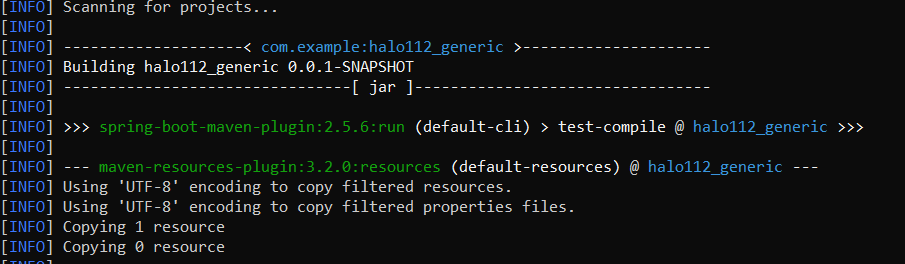
\includegraphics[scale=0.8]{slike/pokretanje_backenda.png}
					\centering
					\caption{Pokretanje backenda iz cmd-a}
					\label{fig:test2}
				\end{figure}
			
			\eject 